\subsection{電流電圧特性}
以下の図\ref{fg:IV_true}にPad型のAC-LGAD検出器の電流電圧特性を示す。横軸が印加電圧で縦軸が暗電流である。
印加電圧を大きくすると、暗電流が急激に大きくなる電圧がある。この電圧は降伏電圧と呼ばれており、電子雪崩起きると暗電流が非常に大きくなるため、このような振る舞いをする。
降伏電圧を超えた電圧だと、ノイズに対しても電子雪崩を起こしてしまい、ノイズが大きくなってしまう。
そのため、LGAD検出器の運転電圧は、ノイズに対して電子雪崩が生じずに、さらに信号の増幅率が最大の電圧に設定することが重要である。
降伏電圧は温度に対して依存性があり、Pad型のLGAD検出器は、1 ${}^\circ$C増加すると降伏電圧が1.1 V増える\cite{Kita_Master}。
温度によって降伏電圧にズレが生じないように、測定の際には温度を一定にする必要がある。
%また、1 ${}^\circ$C増加すると降伏電圧が1.1 V増えるため、電流電圧特性を用いることによって、測定系の温度を調べることもできる。


\begin{figure}[t]
    \centering
    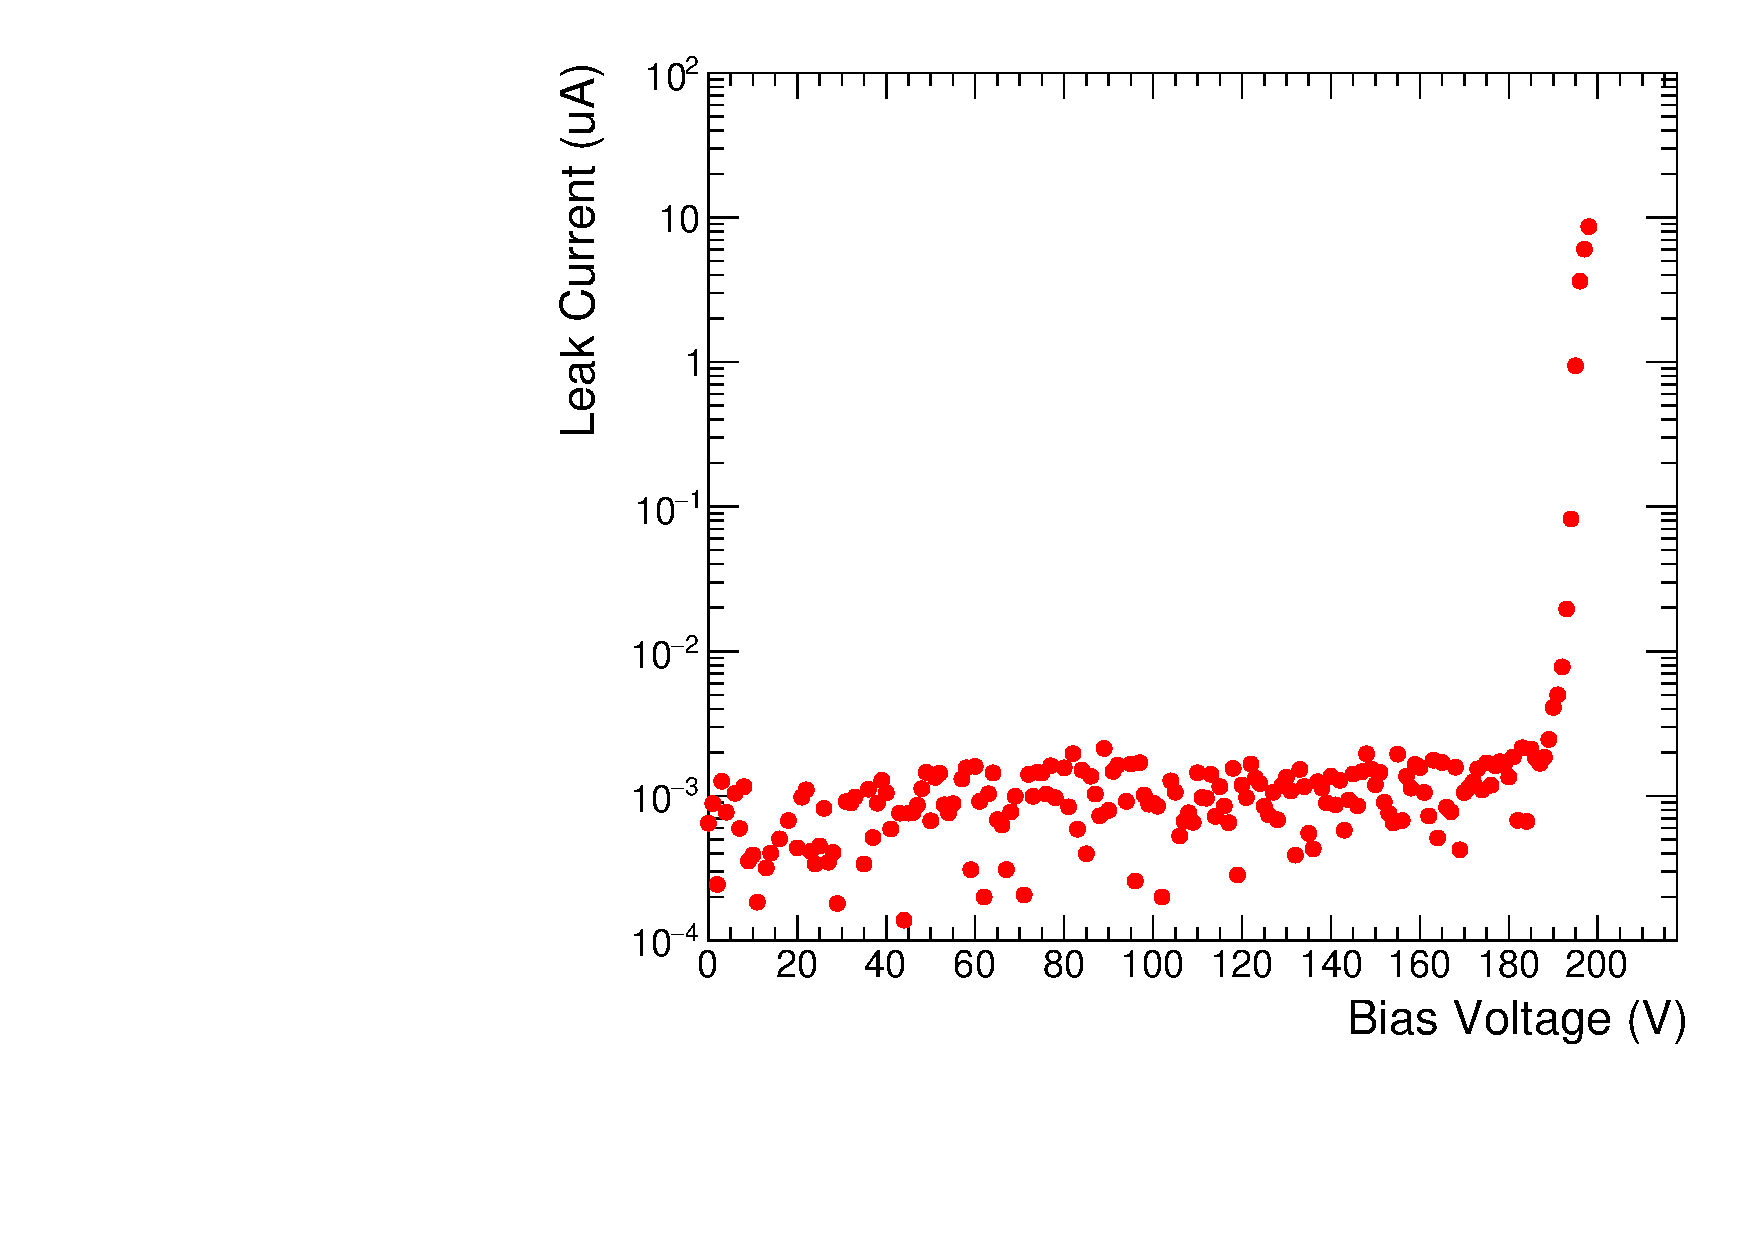
\includegraphics[width=10cm]{fig/graph/IV_true.pdf}
    \caption[Pad型のAC-LGAD検出器の電流電圧特性]{Pad型のAC-LGAD検出器の電流電圧特性\\横軸が印加電圧で縦軸が暗電流、電子雪崩が生じると急激に暗電流が上昇する。}
    \label{fg:IV_true}
\end{figure}